% This is sigproc-sp.tex -FILE FOR V2.6SP OF ACM_PROC_ARTICLE-SP.CLS
% OCTOBER 2002
%
% It is an example file showing how to use the 'acm_proc_article-sp.cls' V2.6SP
% LaTeX2e document class file for Conference Proceedings submissions.
% 
%----------------------------------------------------------------------------------------------------------------
% This .tex file (and associated .cls V2.6SP) *DOES NOT* produce:
%       1) The Permission Statement
%       2) The Conference (location) Info information
%       3) The Copyright Line with ACM data
%       4) Page numbering
%
%  However, both the CopyrightYear (default to 2002) and the ACM Copyright Data
% (default to X-XXXXX-XX-X/XX/XX) can still be over-ridden by whatever the author
% inserts into the source .tex file.
% e.g.
% \CopyrightYear{2003} will cause 2003 to appear in the copyright line.
% \crdata{0-12345-67-8/90/12} will cause 0-12345-67-8/90/12 to appear in the copyright line.
%
%
%---------------------------------------------------------------------------------------------------------------
% It is an example which *does* use the .bib file (from which the .bbl file
% is produced).
% REMEMBER HOWEVER: After having produced the .bbl file,
% and prior to final submission,
% you need to 'insert'  your .bbl file into your source .tex file so as to provide
% ONE 'self-contained' source file.
%
% Questions regarding SIGS should be sent to
% Adrienne Griscti ---> griscti@acm.org
%
% Questions/suggestions regarding the guidelines, .tex and .cls files, etc. to
% Gerald Murray ---> murray@acm.org 
%
% For tracking purposes - this is V2.6SP - OCTOBER 2002


\documentclass[12pt]{article}

\setlength{\oddsidemargin}{0in}
\setlength{\evensidemargin}{0in}
\setlength{\topmargin}{0in}
\setlength{\headheight}{0in}
\setlength{\headsep}{0in}
\setlength{\textwidth}{6in}
\setlength{\textheight}{9in}
\setlength{\parindent}{0in} 

\usepackage{graphicx} %For jpg figure inclusion
\usepackage{times} %For typeface
\usepackage{epsfig}
\usepackage{color} %For Comments
%\usepackage[all]{xy}
\usepackage{float}
%\usepackage{subfigure} 
\usepackage{hyperref}
\usepackage{url}
\usepackage{parskip}

%% Elena's favorite green (thanks, Fernando!)
\definecolor{ForestGreen}{RGB}{34,139,34}
\definecolor{BlueViolet}{RGB}{138,43,226}
\definecolor{Coquelicot}{RGB}{255, 56, 0}
\definecolor{Teal}{RGB}{2,132,130}
%Uncomment this if you want to show work-in-progress comments
\newcommand{\comment}[1]{{\bf \tt  {#1}}}
% Uncomment this if you don't want to show comments
%\newcommand{\comment}[1]{}
\newcommand{\emcomment}[1]{\textcolor{ForestGreen}{\comment{Elena: {#1}}}}
\newcommand{\todo}[1]{\textcolor{blue}{\comment{To Do: {#1}}}}
\newcommand{\pscomment}[1]{\textcolor{Coquelicot}{\comment{Paul: {#1}}}}
\newcommand{\mmcomment}[1]{\textcolor{magenta}{\comment{Max: {#1}}}}
\newcommand{\escomment}[1]{\textcolor{BlueViolet}{\comment{Emma: {#1}}}}
\newcommand{\alcomment}[1]{\textcolor{red}{\comment{Lemmon: {#1}}}}
\newcommand{\hfcomment}[1]{\textcolor{Teal}{\comment{Henry: {#1}}}}
%%%%%%%%%%%%%%%%%%%%%%%%%%%%%%%%%%%%%%%%%%

\begin{document}
\pagestyle{plain}
%
% --- Author Metadata here ---
%\conferenceinfo{WOODSTOCK}{'97 El Paso, Texas USA}
%\setpagenumber{50}
%\CopyrightYear{2002} % Allows default copyright year (2002) to be
%over-ridden - IF NEED BE. 
%\crdata{0-12345-67-8/90/01}  % Allows default copyright data
%(X-XXXXX-XX-X/XX/XX) to be over-ridden. 
% --- End of Author Metadata ---

\title{Developing Beginner-Friendly User Interactions for the Clojure Programming Language}
%\subtitle{[Extended Abstract \comment{DO WE NEED THIS?}]
%\titlenote{}}
%
% You need the command \numberofauthors to handle the "boxing"
% and alignment of the authors under the title, and to add
% a section for authors number 4 through n.
%
% Up to the first three authors are aligned under the title;
% use the \alignauthor commands below to handle those names
% and affiliations. Add names, affiliations, addresses for
% additional authors as the argument to \additionalauthors;
% these will be set for you without further effort on your
% part as the last section in the body of your article BEFORE
% References or any Appendices.

\author{
Henry Fellows, Aaron Lemmon, Max Magnuson, \\
	Emma Sax, Paul Schliep, and Elena Machkasova \\
Computer Science Discipline \\
University of Minnesota Morris\\
Morris, MN 56267\\
fello056@morris.umn.edu, lemmo031@morris.umn.edu, magnu401@morris.umn.edu, \\
	saxxx027@morris.umn.edu, schli202@morris.umn.edu, elenam@morris.umn.edu
}
\date{}
\maketitle
\thispagestyle{empty}
%\alcomment{Should these say @morris.umn.edu?}

\section*{\centering Abstract}
The abstract
\escomment{Is this supposed to be the abstract that we submitted? The
  one that's three paragraphs long?}
\emcomment{No, usually it's different from the abstract submitted for
  review. An abstract is usually written when the paper is nearly
  finished.}

\newpage
\setcounter{page}{1}

\section{Introduction and Background}\label{sec:intro}
Felleisen et al~\cite{Felleisen:2004} have made an excellent case for
using a Lisp as a programming language in an introductory CS class:
the first language new programmers will use. Lisp offers a simple
syntax and introduces students to modularity, abstraction, and
data-driven program design while developing good programming
practices being explicit about program design principles.
Essential concepts taught in such an
introductory class have been shown to be effective in building a
strong foundation that allows students to
build upon in later classes that introduce imperative features and 
object-oriented paradigm~\cite{Bieniusa:2008}. 

Clojure is a relatively new language in the Lisp family that is
rapidly gaining popularity in industry and in the open source
community. Clojure provides a functional easy-to-use approach to
developing robust multi-threaded programs. 
 
Clojure offers a variety of built-in datatypes and
functions that, when introduced rigorously and systematically in an
introductory CS class, would allow students to practice data-focused program
development. The abundance of open
source libraries and projects allow students to continue development
in Clojure after finishing the introductory course, both for their own
purposes (such as data processing for other courses) and as
contributions to projects of others.  

This paper describes our work in progress in making Clojure and its
environment usable for introductory level students. Our efforts
include transforming Clojure error messages into more
beginner-friendly ones and developing tools that would allow students
to seamlessly run their program code integrated with our
modifications without having to deal with Clojure tools that require
more advanced knowledge. 

\subsection{Overview of Clojure}\label{sec:clojure}
%\emcomment{Emma - many thanks for getting things started! Below are
%  comments. The majority of them refer to making this material
  %understandable to the target audience (i.e not using terms that
  %CSci undergrads typically don't know. Otherwise things are well
  %organized and well written.}
  
  
Clojure, developed in 2007 by Rich Hickey~\cite{Hickey:2008}, is a dynamic, functional
programming language in the Lisp family.
Dynamic typing means that Clojure does not associate types with variables, but rather with values that they contain.
When a type of a value is inconsistent with one expected in a given context, a runtime error occurs.
Functional means
that Clojure functions are first-class values that can be passed as arguments and returned
as values.
%Also, Clojure code does not change state.
%\emcomment{need to be more precise here; also probably need to explain what ``functional'' means.}
%\emcomment{``dynamic'' refers to ``dynamically typed''} 
%\emcomment{Use simpler, more concrete terminology: there are many ways
  %in which JVM can be utilized. Probably need to explain that the JVM
  %is Clojure interpreter, mention and explain REPL somewhere in this paragraph.}
%\emcomment{Need to explain what you mean by dynamic}
Clojure utilizes the Java Virtual Machine (JVM) as a runtime environment. Clojure compiles into Java bytecode
and runs on the JVM, which abstracts over the specifics of the hardware.
%\hfcomment{It's a runtime enviroment - the bytecode is compiled and it runs on the JVM, which
%abstracts over the specifics of the hardware.}
This setup offers easy 
%\emcomment{accessibilty?} 
access to Java frameworks. The Clojure read-eval-print loop (REPL)
%\emcomment{what does REPL stand for?} 
is another easy way to interact 
%\emcomment{to interact with Clojure?}
 with Clojure. A REPL is an interactive shell program that takes single 
expressions, evaluates them, and returns the result to the user. The REPL allows users to see 
immediate results and respond easily and quickly. For any programmer, the use of the REPL 
is highly advised and can make programming in Clojure much simpler. Use of the REPL allows users
to break down their code, test specific pieces, and experiment with new functions and uses~\cite{clojure-REPL}.
%\emcomment{explain why?}
%\emcomment{This wouldn't make any sense to the target audience and is
  %not needed (perhaps with the exception of multithreading:}
%including optional type hints
%and type inference and easy multithreading options. All the while,
%Clojure remains completely dynamic.  
%\emcomment{This is a strange wording: what does it mean to ``remain''
 % in this context? And you already said it was dynamic.}

Because Clojure is a functional language, it puts strong emphasis on
immutable data types. An immutable data type means data cannot 
%\emcomment{data cannot be changed, not data types}
be changed. When using Clojure, in order to change a data item, an entirely 
new data item must be made. Immutable data types help prevent side effects in programs. 
A side effect is when a function alters memory outside of its scope. Side effects can make 
debugging or resolving errors more
difficult. This is because when a function interacts with other parts of a program,
%\emcomment{with other parts of a program} 
when it is not supposed to, any issues in the code can propagate throughout the program. The
reduction of side effects makes problems with the code are easier to find and fix.
Because of this, immutable data types are practical for novice programmers.
%\emcomment{I would first explain what side
  %effects are, and only then why they complicate things for novice
  %programmers}
  
Clojure, like other Lisp languages, uses prefix notation. This means
that function calls use parenthesis, followed by the function name,
and then any parameters: 
\begin{verbatim}
	(<function-name> <argument 1> <argument 2>)
\end{verbatim}

An example of this can be seen through addition, which is a built-in function, unlike traditional
languages where \texttt{+} is an operation: %a built-in mathematical function, addition:
% \emcomment{All functions, including built-in mathematical functions, use this form? ``Even'' implies
%that somehow this is unexpected.} built-in functions, such as mathematical functions, use this form:

%\hfcomment{I'd explicitly note that + is not an operation, as in C or Java. It's implied, but it's
%just easier to bludgeon your reader into submission.}
\begin{verbatim}
	(+ 5 5)
	-> 10
\end{verbatim}

Note that \texttt{->} indicates the result of computations in the Clojure interpreter.
%\emcomment{We indicate the result of computations in Clojure
  %interpreter as \texttt{->} -- plus we need to explain REPL and
  %interpreter.}

%\emcomment{I don't think we need syntax for interop. I would comment
 %out the example for now.}
Clojure also has offers accessibility to Java functions and Java
interoperability. This means that any Java method can be called just
like normal Clojure functions.
%\begin{verbatim}
%	(.methodName object *arguments)
%\end{verbatim}

%\emcomment{Thsi is true, but probably not useful for our readers}
%As well as the use of Java methods, Clojure can also use macros, Java
%utilities, concurrency and multithreading, and even certain Java
%objects to enhance the abilities of using Clojure. 

%\emcomment{before we get into anonymous functions, we need to show how
%to define regular functions (general syntax and a couple of examples)}
Clojure users can also define functions and variables.
%\emcomment{I don't think we need to explain why people name functions}
Using the keyword \texttt{def}, we can define variables:
%\emcomment{this is a confusing way of saying it, especially because what you are showing is not a
%function. How about just talking about defining variables? (and technically functions are values
%anyway, just like numbers and strings }
\begin{verbatim}
	(def mystring "Hello World")
	mystring
	-> "Hello World"
\end{verbatim}

In the above example, we define a variable to hold the string to be \texttt{"Hello World"}. This way,
whenever we reference 
%\emcomment{I would avoid ``call'' here since calling is for functions} 
\texttt{mystring}, the string we bound to the variable name will be returned. We can also use
\texttt{defn} to define functions:
%\emcomment{need to say that defn is used for defining functions}
\begin{verbatim}
	(defn increment-number [number] (+ number 1))
	(increment-number 2)
	-> 3
\end{verbatim}

In this example, we defined
%\emcomment{define} 
a function that takes a number and returns that number incremented by 1.
%\emcomment{returns that number incremented by 1}. 
In any function, the function name is the word after the \texttt{defn}, the pieces in the square
brackets after the function name indicate the function's parameters, and what follows is the body, 
which is the expression returned by the function.
%\emcomment{the expression that the function returns ("action" sounds imperative)}. 
%\emcomment{the expression returned by the function? ``does'' has imperative flavor}

Now let us say that we have a program where we want to use a function, but only once. This means that
we do not necessarily need to define it with a name because Clojure supports anonymous functions.
Anonymous functions allow programmers to quickly define functions in place
% \emcomment{not sure what you mean by``rare'' here. Those that aren't predefined?}  
when needed. 
However, since these functions are not  stored, the program would not be able to use them more than
once. 
%\emcomment{call them?} by name after the usage. 
The following example is of the same increment-number function as above, but implemented anonymously.
The \texttt{map} function takes in a function and a collection as arguments, and applies the function
to the collection: 
\begin{verbatim}
	(map (fn [number] (+ number 1)) [0 1 2 3])
	-> (1 2 3 4)
\end{verbatim}
%\emcomment{Give an example of using an anonymous function}

%In anonymous functions, anything in the brackets that is following the
%\texttt{fn} is arguments. 
%\emcomment{and in regular functions as well} 
%After the arguments in \texttt{[]}, is the
%body. If the program wanted to be able to call this function multiple
%times, it would make more sense to simply put a \texttt{def} with a
%name in front: 
%\emcomment{It's not quite that: firstly, it's defn, and not def, but
 % you also need to explain where the function name is}
%\begin{verbatim}
%	(def increment-number [number] (+ number 1))
%\end{verbatim}

%Now, the program can call this function any time by using the name \texttt{increment-number}.

Clojure also has a variety of different types of data structures, also referred to as collections. All 
of Clojure's collections are immutable, which means that the data within the structures cannot be
modified. 
%\emcomment{I wouldn't go into persistent, just talk about immutable.}
%This means that the data in the structures cannot be modified, and that each
%structure preserves the previous version of itself. 
The different types of structures Clojure uses are lists (denoted by \texttt{()}), sets (denoted by
\texttt{\#\{\}}), vectors (denoted by \texttt{[]}), and hashmaps (denoted by \texttt{\{\}}). The first
three types of data structures mentioned can contain any number of values of any data type.
%, including \texttt{nil} (Clojure's equivalent of \texttt{null} or nothing), of values. Data
%structures are untyped. This means that a collection may contain any data type. 
%\emcomment{too informal, rephrase} if types of values in one structure
%mismatched):
%\mmcomment{I think that the above sentence should make it more clear that a collection may contain any
%data type. Maybe, don't mention numbers and stick to data types?}
%\emcomment{agree}
%\emcomment{don't use the word ``normal'' in a research paper} data structures: 
\begin{verbatim}
	(1 2 "foo" :a 9 "bar")
\end{verbatim}

%\emcomment{I am not sure which of data structures we will actually need; we
  %never defined keywords, and I am not sure we will need those (but if
  %we do, we will need to explain them). We will definitely need
  %vectors and lists and hashmaps. Sets probably not.}

%They \emcomment{Not sure what ``they'' referes to; most structures can
%hold any amount (any number, to be more precise) of values, nil isn't
%explained, and probably needs to 
%be, but I am not sure; nil isn't an amount of anything.} can hold any
%amount, including \texttt{nil}, of values of any type 
%\emcomment{we need to mention earlier that all data structures are
 % untyped: not unique to hashmaps}
%(a data structure is untyped, which means it does not care if
%types of values in one structure as mismatched).

However, hashmaps are unique in the fact that it is a collection of key-value pairs: 
\begin{verbatim}
	{key value, key value, key value}
\end{verbatim}

Hashmaps commonly use keywords. Keywords are simple names that have a colon in front.
An example of a hashmap using keywords follows: 
%\emcomment{why ``realistic''? Just an example. What you are showing above is abstract syntax} 
\begin{verbatim}
	{:a 1, :b 2, :c 3}
\end{verbatim}
%\emcomment{It's unclear from just the syntax what it means to be a
%  collection of key/value pairs.}

%\emcomment{I would first introduce keywords and then explain that they are typically used as keys}
%\emcomment{Introduce keywords as a datatype before you first use them in an example (perhaps before
% collections)}
The keywords in the above hashmap are: \texttt{:a}, \texttt{:b}, and \texttt{:c}. Keywords, such as the
ones above, are often used as keys within hashmaps. The value is the second piece of a key-value pair,
and each value is bound to a key. In the above example, \texttt{:a} is bound to \texttt{1},
\texttt{:b} is bound to \texttt{2}, and \texttt{:c} is bound to \texttt{3}.
%.  Keywords, such 
%In hashmaps, usually keywords, indicated by a colon in front of a
%simple indicating word, are used as keys, and the value is what the
%key is bound to. 
%\emcomment{keys aren't pointing to anything, they are bound to something}
%In the hashmap above, the keywords are

Just like all other values, data structures can also be bound to a
variable name: 
\begin{verbatim}
	(def myhashmap {:a 1 :b 2 :c 3})
	myhashmap
	-> {:a 1, :b 2, :c 3}
\end{verbatim}

Laziness is another common feature of Clojure. Laziness is when the evaluation of an expression is
postponed until the return value is needed. An example is the Fibonacci sequence.
It would be impossible to store all of the infinite numbers in the Fibonacci sequence. By making a lazy
function, Clojure can
evaluate only as much of the Fibonacci sequence as necessary. The next example illustrating laziness 
uses the functions 
\texttt{take} and \texttt{range}. \texttt{take} takes the first $n$ elements of a collection, both of
which are given as arguments. \texttt{range} returns an infinite sequence of non-negative
integers, beginning at 0:
\begin{verbatim}
	(take 10 (range))
	-> (0 1 2 3 4 5 6 7 8 9)
\end{verbatim}

Another common example of laziness are \texttt{if} statements:

\begin{verbatim}
	(if (< number 10) (+ number 1) (- number 1))
\end{verbatim}

In the above example, the \texttt{(+ number 1)} or \texttt{(- number 1)} only evaluates depending on
whether the \texttt{(< number 10)} evaluates to true or false.

The opposite of a lazy evaluation is an eager evaluation. Eager evaluations fully evaluate their
parameters collection upon runtime.

%This enables the data structures to be called, traversed, etc by the
%use of a single name. \emcomment{I am not sure this addds anything; an
%example would be better.}

\subsection{Overview of ClojurEd project}\label{sec:project}
ClojureEd is a project at UMM that is devoted to increasing usability
of Clojure in an educational setting, in particular in introductory
classes. It has originated in 2013 as a joint effort of alumni,
students, and faculty. Several students have contributed to it as a
part of several research efforts, in particular as a part of a two
months summer research program in 2014 sponsored by the HHMI (Howard
Hughes Medical Institute) grant and UMM MAP (Morris Academic Partnership). Two
other students are currently working on the project sponsored by UMN
UROP (Undergraduate Research Opportunity Program). 

As a part of the project we have developed the system of modifying
Clojure error messages, as described in section~\ref{sec:errors}. The
current challenges involve integrating our system with 
Clojure project management tools and IDEs. The summer project explored
some approaches to this problem, but did not result in a
solution. Recently we have identified elements of the Clojure project
architecture that would allow us to develop plugins to handle student
code in a way that would not require any advanced knowledge (such as
working with command line) on their part. However, this is still work
in progress, and no working solution exists at this
point. Section~\ref{sec:technical} details these efforts and
challenges. 

The code is available at

\noindent
\url{https://github.com/Clojure-Intro-Course/clojure-intro-class} 

\section{Error Messages}\label{sec:errors}

\subsection{Current error messages in Clojure}\label{sec:currentem}
Error messages are an important part of programming since they are the main source of communication between a user and the 
system when an error occurs in the program.
Error messages are especially important for introductory programmers who have had little to no experience with troubleshooting 
programs. %\emcomment{programs?}
These error messages need to provide helpful and easy-to-understand information that can be used to resolve issues.
%\emcomment{The two sentences are very similar and should be merged}

Error messages in Clojure are not particularly useful for introductory programmers because they do not provide information that 
can help guide a student in fixing the error.
Also, Clojure error messages are typically complex because they originate from the underlying Java interpreter (JVM), which most 
%\emcomment{most} 
novice programmers will be unfamiliar with.
Below are some examples of error messages in Clojure that might be unhelpful or unintuitive for an introductory student.

\subsubsection{Example 1}\label{sec:ex1}

Consider the following (erroneous) code fragment:
%\emcomment{Consider the following (erroneous) code fragment:}
\begin{verbatim}
(defn square-this (* input input))
\end{verbatim}

In this code sample, the programmer is attempting to create a function \texttt{square-this} which will take a number and return 
the square of its value.
However, the programmer forgot to declare that \texttt{input} should be a parameter.
In Clojure, function declarations always require a vector containing the declared parameter names.
The resulting error message is: 
\begin{verbatim}
IllegalArgumentException Parameter declaration * should be 
a vector 
clojure.core/assert-valid-fdecl (core.clj:6842)
\end{verbatim}
It does provide key words that could lead the programmer to fixing the issue such as \texttt{Parameter} and \texttt{vector}.
However, the error message also includes information that a new programmer might find intimidating or confusing such as 

\noindent
\texttt{clojure.core/assert-valid-fdecl (core.clj:6842)}.



The error can be corrected by placing a vector of inputs, in this case containing a single input, right 
after the function name.
%\emcomment{The previous sentence creates an awkward flow. Maybe "the error can be corrected by placing 
%a vector of inputs, in 
%this case containing a single input, right after the function name"?}
Here is an example of the code above after corrections have been made:
%Corrected Code:
\begin{verbatim}
(defn square-this [input] (* input input))
\end{verbatim}

\subsubsection{Example 2}\label{sec:ex2}

In the next example, the programmer is attempting to return a new hashmap with an added key-value pair.
The function \texttt{assoc} is generally used to make this happen.
\begin{verbatim}
(assoc :a 3 {:a 5, :b 8, :c 9})
\end{verbatim}

In this attempt, the programmer did not put the arguments for \texttt{assoc} in the correct order.
When using the function \texttt{assoc}, the hashmap should go before the new key and value.
The error message that results follows:

\begin{verbatim}
ClassCastException clojure.lang.Keyword 
cannot be cast to clojure.lang.Associative
clojure.lang.RT.assoc (RT.java:702)
\end{verbatim}

Since Clojure expects the first argument to be a hashmap and it is not, it tries to cast 
the keyword \texttt{:a} into a hashmap.
This error message refers to \texttt{clojure.lang.Associative}, which is actually a Java interface.
%\emcomment{it also refers to typecasting which is unfamiliar to Clojure users since Clojure is 
%dynamically typed with no explicit type declarations.}
Referring to that interface may not be useful for Clojure programmers if they have little to no 
experience with Java or type hierarchies.
Furthermore, the error message refers to typecasting, which is unfamiliar to Clojure users since 
Clojure is dynamically typed with no explicit type declarations.
The error message is ineffective at explaining to the programmer that the underlying problem with their 
code was a misordering of arguments.
Here is an example of the code above after corrections:
 
\begin{verbatim}
(assoc {:a 5, :b 8, :c 9} :a 3)
-> {:c 9, :b 8, :a 3}
\end{verbatim}

%\emcomment{You might want to talk about the message transformations first, and then user scenarios used to test how well it works}

\subsection{Error message transformations}\label{sec:transform}

Since standard Clojure error messages are generally unhelpful, we aim to replace many Clojure error messages with improved ones.
%\emcomment{via a {\tt try/catch} statement}
%\emcomment{substitute them with?} our replacement messages.
A way of accomplishing this is by reading in a user's code and wrapping it in a \texttt{try/catch} block.
Then any errors thrown by the user's code will be checked against a large collection of regular expressions.
If a regular expression matches, important details from the original error message are captured and used to insert details into our replacement message.
However, this \texttt{try/catch} approach does not work well in all situations.
Additional technical challenges arise when dealing with compiler exceptions, the REPL, and lazy sequences.
Section~\ref{sec:technical} discusses the implementation details and current progress in more detail.
%\emcomment{Need to mention that in a simple case this approach means surrounding student code with  a {\tt try/catch}. However, this simple approach is not sufficient for Clojure. Section~\ref{sec:technical} discusses the implementation details and challenges.}


%\emcomment{I would start by describing the try/catch/replace approach, and only then talk about replacements. Replacements are 
%there to determine specific arguments (5, "hello", etc) and report those to the user.}

%An alternate way we replace Clojure error messages is through function substitution.
In the case of predefined functions, such as \texttt{map}, we achieve more informative error messages through function substitution.
This involves defining functions with the same name as standard Clojure functions.
Within these definitions, we can do type checking on arguments passed in.
If the type checks find an error, our system displays a customized error message.
If no type errors are found, the arguments are passed on to the actual corresponding Clojure function.
Although this method can only handle runtime exceptions, it is advantageous because we can capture the actual values of the 
arguments passed in to the redefined functions and use them to provide a detailed error message. As an example, consider the following erroneous code:

\begin{verbatim}
(map "add one" [1 2 3])
\end{verbatim}

Clojure provides the following error message:

\begin{verbatim}
ClassCastException java.lang.String cannot be cast to
clojure.lang.IFn  clojure.core/map/fn--4245 (core.clj:2557)
\end{verbatim}

Our function substitution error handling displays a more informative message:
\begin{verbatim}
ERROR: In function map, the first argument "add one" must be
a function but is a string.
\end{verbatim}

This message provides information that the problem occurred in the first argument, the offending argument's value was ``add one", and that the argument was a string instead of a function. While function substitution is cumbersome because it involves redefining each function individually, it is the only way to provide the user with specific information about which arguments are causing the problem.


Both the \texttt{try/catch} and function substitution methods together, unfortunately, do not handle all possible cases.
For example, complexities arise when students define their own functions, especially if they are anonymous functions.
We are unable to anticipate the function definitions that users of our system create, so we cannot rely on function substitution 
for those cases.
The \texttt{try/catch} approach must handle those scenarios.
Replacement error messages are even harder to make for anonymous functions since they have no name by which we can refer to them.
Although our system does not handle all cases, we hope that it will be helpful in the majority of cases that a Clojure programmer 
will encounter.

%\alcomment{add a paragraph explaining that this does not handle every possible case. For example, complexities arise when 
%students define their own functions, especially if they are anonymous functions. However, we hope that our system will be 
%helpful in the majority of cases that it does handle.}

%\pscomment{Should we include an image of the error popup of our system?}

\subsection{User scenarios}\label{sec:scenarios}

In order to better understand what our software users might encounter, we developed user scenarios detailing typical coding 
problems a new programmer might face.
To create these user scenarios, we created solutions to common beginner programming exercises and purposefully introduced errors 
that a new programmer might make.
We then recorded the error messages that these solutions produced.
We also took note of the underlying cause of the errors so that we have a better idea of how to improve upon the error messages 
for our program.
We then took the same solution and ran it within our program to compare the error message our system produces against the one 
Clojure produces.

These user scenarios showed us typical errors a student will be experiencing when learning to program in Clojure for the first 
time.
For example, when a student first starts writing basic operations in Clojure, a typical mistake might be forgetting to put the 
function in front of the arguments,
such as \texttt{(5 - 5)}, where it should be \texttt{(- 5 5)}. 
This produces a message that would be unhelpful for introductory programmers: 

\begin{verbatim}
ClassCastException java.lang.Long cannot be cast to
clojure.lang.IFn user/eval769 (core.clj line 675)
\end{verbatim}

In this error message, \texttt{clojure.lang.IFn} is a Java type representing Clojure functions. So, the error message is 
actually saying that 5 is a number, not a function, since Clojure expected the function name to be listed first. Our system 
produces the following error message to replace the one above:

\begin{verbatim}
ERROR: Attempted to use a number, but a function was
expected. intro.core/-main (core.clj line 675)
\end{verbatim}

%\emcomment{Perhaps explain that clojure.lang.IFn is a Java type for Clojure functions, thus the error message is saying that 5 
%is a number, not a function}
%\emcomment{I am still thinking of user scenarios as ways of evaluating our new messages compared to the Clojure standard messages, so 2.2 and 2.3 should be switched}

\subsection{Future work: hints}\label{sec:hints}

While the error message our system produced above says what the core problem is, it does nothing to suggest to the user to check 
that the arguments are in the correct order, which is the fundamental issue.
We are developing a system of hints that offer additional guidance in figuring out why errors have occurred.
Hints are suggestions shown to the user along with an error message.
Since there is no sure way of telling exactly what went wrong, we will offer several hints that may be applicable to the 
situation.

For example, a \texttt{ClassCastException} is usually thrown when programmers place arguments in an incorrect order.
However, a \texttt{ClassCastException} can be thrown in many other cases as well, which can make providing a specific hint challenging.
Thus, our system provides several hints in order to cover a variety of situations.
Hopefully, one of the suggestions will be helpful in solving the real issue.

Developing user scenarios was a helpful exercise because it allowed us to immediately know the root cause of an error even before 
seeing the error message.
This allowed us to easily record a human interpretation of the problem and relate it to the error. This process gave us a useful 
methodology for creating hints. As an example, the following user scenario involves a hypothetical attempt to write a program that 
would print ``Hello World":

\begin{verbatim}
(print Hello World)
\end{verbatim}

This results in the Clojure error message:
\begin{verbatim}
CompilerException java.lang.RuntimeException:
Unable to resolve symbol: Hello in this context
\end{verbatim}

Our hint for this may be more informative and educational for a new programmer than the error message above:

\begin{verbatim}
It looks like Clojure is expecting that Hello is something
named in your program. If you wanted Hello and any following
words to be plain text, try surrounding them with double
quotes. If Hello is referring to something named in your
program, make sure it is spelled correctly.
\end{verbatim}

User scenarios provide a useful methodology for generating hints, which we will continue to use to extend the system.
We plan to work with Clojure beginners interactively to improve the hints in the system.
We also plan to provide links to Clojure documentation when appropriate in the hints.
Once beginner programmers are comfortable with the terminology used on the documentation pages, directing them to the documentation will provide them with a more concrete understanding of the language.


\section{Technical Setup}\label{sec:technical}

In our prospective error handling, there are a large number of technical issues. First we need to figure out how to catch and process the errors. Then, we need to figure out how to integrate that system with the tools for managing Clojure projects. Throughout this process it is important to be mindful of usability for introductory students. Therefore we would like to synthesize the error handling system and the tools used by the student in a way that is both usable and robust. The system as a whole is a work in progress; the development and choice of tools takes a significant amount of time. We spent our time exploring tools and how to implement them. We decided that we would like to avoid altering the code of the tools themselves, instead we would like to develop plugins that would provide the functionality that we need. 

\subsection{On the nature of errors in Clojure}

%\emcomment{Move to beginning, then talk about errors}
%\emcomment{just make a reference back to 1.1 where we have introduced REPL: the explanation of why it is useful should be there, 
%not here}
%\emcomment{A side note: and when running expectations}
There are two different environments where code can be evaluated in Clojure. A user can evaluate all of their code by running it, or they can evaluate code snippets using the REPL. When developing code, it is common practice for a user to use REPL to test pieces of their code. This is practice is described in depth in section \ref{sec:clojure}. Due to the importance of REPL interactions for code development and debugging, it is essential for the errors in both environments to be consistent. Therefore, we need to make sure that our error handling system is capable of addressing the errors from compilation, runtime and REPL.

%\emcomment{a minor note: since compilation errors happen first, mention them first? Also mention that due to a dynamic nature of Clojure many type errors that would've been compilation errors in Java are runtime errors in Clojure}
%\emcomment{they don't stem from laziness, their timing is affected by laziness; also note that running code in REPL also presents challenges even for runtime errors}
%\emcomment{laziness seems to be spelled with an i}
In Clojure, error messages are divided into two different categories, compilation time and runtime. As their names imply, compilation errors occur when the code is compiled, and runtime errors occur when the code is run.
Compilation errors cannot be handled by a simple {\tt try/catch} because they originate in the compiler before the code is even evaluated. Therefore, we need to catch the errors from the compiler so that we can handle them. The compiler errors common in Java shift to runtime errors in Clojure, because the types in Clojure are dynamic and are thus checked at runtime.
Handling runtime errors is made relatively simple by using a {\tt try/catch} with the exception of handling errors that involve laziness. Since lazy sequences are evaluated when they are needed, an error in a lazy sequence will not occur until the sequence needs to be evaluated. This means that the error will often not occur where it originated. When this is the case, the user will be provided with unhelpful or often misleading error messages about the nature of the problem. These errors can be very frustrating to troubleshoot especially for introductory students. %Compilation errors are much more difficult to handle than runtime errors. 
%\emcomment{I think you are going into a lot of technical details that should be explained on the diagram. Also make it clear that we have solved some of these challenges, but for many (most?) of them this is still a work in progress.}

None of these problems have not been resolved, but we have determined approaches that should solve these problems. Finding the origin of errors caused by laziness has not been solved, but we have a potential solution that involves forcing evaluation of lazy sequences in student code. Compilation errors are also problematic, but we hope to resolve this by intercepting error messages as they are created, which is detailed in section \ref{sec:approach}.
 
\subsection{Leiningen}
Leiningen is an open source project under active development that is the primary tool for project management in the Clojure community\cite{LeinGitHub}. Leiningen is a fully featured project manager that cleanly deals with dependencies as well as provides useful tools for developing projects. When a project is run in Leiningen, Leiningen will resolve all dependencies. For example, if your project requires a plugin, Leiningen will automatically retrieve, install, and apply that plugin to your code. After it has resolved the dependencies, Leiningen uses other tools to build, compile, and run the project. Leiningen makes running Clojure projects extremely simple for the user. With Leiningen, it only takes one command to begin a new project, and it only takes one command to run a project. Because of the level of abstraction that Leiningen offers, we have decided that it is the best option for an introductory course.

While Leiningen is a very helpful tool, there are still some aspects that are challenging for introductory students. The most difficult of which is the interface. Leiningen uses the command line as its primary interface. The command line is both a distraction and a barrier to teaching the material in an introductory course. Therefore, we would like to abstract over the command line by using a graphical interface, ideally integrated with the IDE used by students. This graphical interface would extend the simplicity of Leiningen while still providing the same functionality needed by students.

\subsection{IDEs}
\mmcomment{We still need references for this section.}
Choosing the right IDE is important, especially for an introductory class, because it is the environment in which students will develop their code. We have looked into many of the IDEs available for Clojure, and we have decided that the most promising choices are LightTable and Nightcode. Both IDEs offer intuitive interfaces, syntax checking, built-in REPLs, and easy project management. They each use Leiningen to build projects, but neither of them provides a complete integration with Leiningen. Users still need to use the command line for some functionality. They are also both maintained by open source communities and are under active development. This allows us to take advantage of new features and modifications developed by others.  

Both IDEs have a lot of functionality that we are looking for, but they do have some notable differences. For instance,  LightTable requires a separate installation of Leiningen. This adds another layer of difficulty for the student since installing Leiningen is non-trivial. Nightcode comes packaged with its own distribution of Leiningen. This makes Nightcode easier to install and use. The REPL differs between
 each IDE. In LightTable, the user opens up REPL using a context menu, and the REPL constantly evaluates each line of code in it. This ultimately provides more information, but it is very different from the traditional REPL in ways that may be a little confusing for introductory students. In Nightcode, the REPL will always up in a
  separate frame, and each line is only evaluated when the user hits enter. LightTable uses hot keys and a context menu to do a lot of the tasks in LightTable such as running the project or
 starting a REPL. This is less familiar to introductory students, and it may be a little daunting at first. LightTable does provide a nice easy reference for searching for the appropriate hot keys to lessen the learning curve. Alternatively, Nightcode
 uses a lot of clearly labeled buttons and tabs that are intuitive for the user to perform tasks. Since it is unclear which IDE will be more common in the Clojure community in the future, we plan to support both options.

%\mmcomment{Do we have a preference for either or which one will likely be used in the introductory course?} 
%\emcomment{You kind of made the case for Nightcode here. Perhaps make it more clear what the advantages of LightTable are? 
%Ultimately, however, we are trying to target both because wer don't know where the community will go a few years down the road 
%(see my comment above)}

\subsection{Approaches}\label{sec:approach}
%\emcomment{Use consistent capitalization in section titles}
%\mmcomment{Describing the journey to nREPL}
%\mmcomment{Is this section necessary?}

Our first approach was to develop an IDE-specific plugin to intercept the error messages going to the console of the IDE. We discovered that it was not the IDE that was directly interacting with the compiler. Our next approach was to use a Leiningen plugin to try and intercept error messages. We searched through the Leiningen source code, and attempted various methods of interacting with Leiningen. None of these approaches allowed us to intercept the error messages that were being printed to the console. We have determined that Leiningen uses nREPL, which is a Clojure interpreter, to handle compilation and error messages.

The nREPL interpreter is a client-server system for evaluating user code. nREPL middleware can intercept messages from the nREPL system and apply functions to those messages. nREPL middleware uses handlers for interacting with the messages. These handlers look for operations with certain keywords and only are applied to those specific operations. For example, an nREPL middleware can specify a handler for evaluation operations. The middleware will inspect every operation that passes through nREPL. If it is an evaluation operation, then the functions specified in the middleware will be applied to the operation. If the operation is not an evaluation function, then nothing will be changed.

Now, our planned approach is to write an nREPL middleware to intercept the error messages handled by nREPL and clean them up. 
This approach is also preferable to our initial IDE specific approach because it allows for our system to be IDE independent. 

\subsection{Implementing error handling}

\begin{figure}[h]
 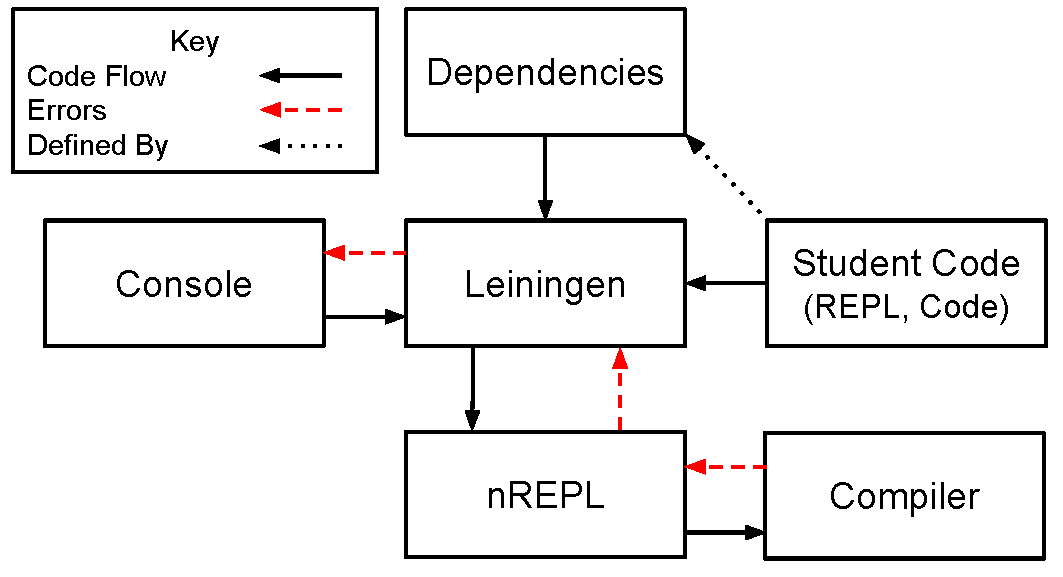
\includegraphics[width=12cm]{CurrentErrorHandling.pdf}
 \centering
 \caption{Workflow diagram of running a Clojure project in Leiningen}
 \label{fig:CurrentError}
\end{figure}

%\emcomment{I see a compiler here, but I don't see an interpreter. Is nREPL an interpreter? Make it clear}
%\hfcomment{There are no interpreters in canonical Clojure.}

The current error handling system is described by figure \ref{fig:CurrentError}.First, the student runs their project through Leiningen using the console by calling \texttt{lein run}. Then, Leiningen will take the dependencies defined in the student code and resolve them. After the dependencies have been resolved, Leiningen then sends the code to nREPL to be compiled and evaluated. Any errors are passed back to the current output device, which is the terminal by default. 

%\emcomment{where? can you show it in the diagram?}
%\emcomment{replace? Transform?}
%\emcomment{address the difference between compilation errors and runtime errors since you mentioned those earlier; also mention 
%where REPL interactions happen in this setup.}
In our approach, we would like to catch the errors from nREPL by using nREPL middleware. Once we catch those errors we will 
transform them as described in section \ref{sec:errors}. After being cleaned up, the error will then be rethrown to Leiningen, so 
that it can be printed out for the student to see. We believe that nREPL handles all errors thrown by the compiler, runtime, and 
the REPL. The middleware will then handle all of these cases in a consistent manner.

\hfcomment{Fig 2 goes here.}
\begin{figure}[h]
 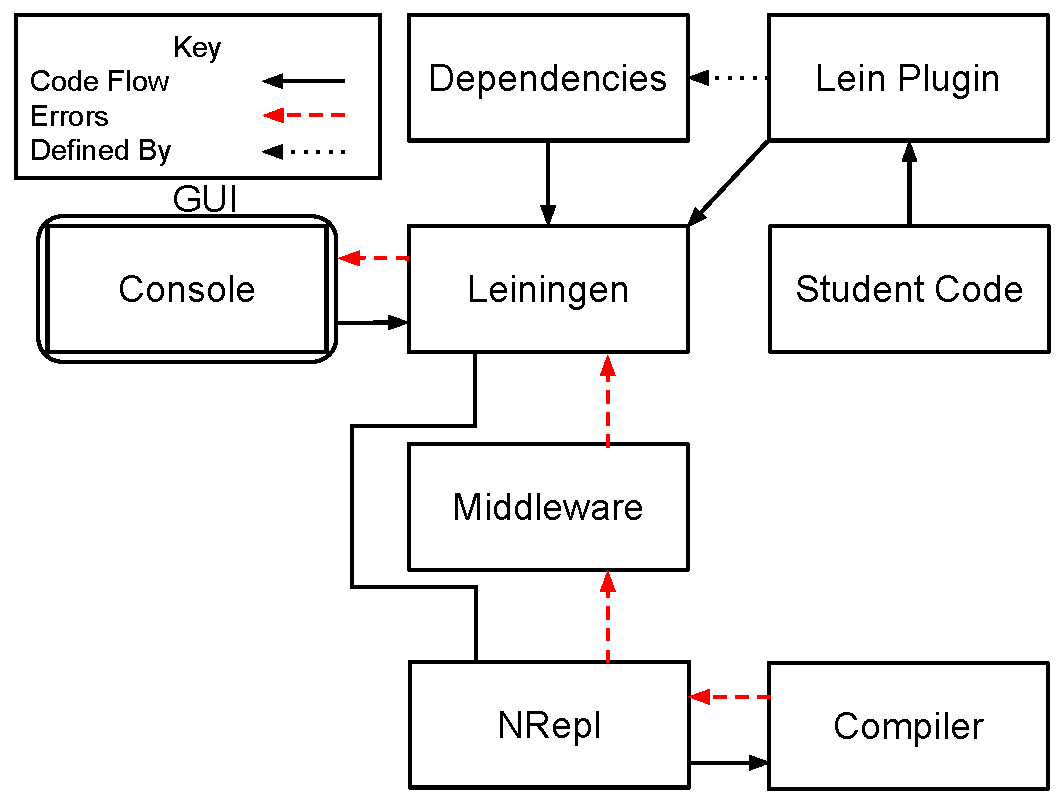
\includegraphics[width=12cm]{OurErrorHandlingSystem.pdf}
 \centering
  \caption{Planned workflow for our error handling system}
 \label{fig:OurSystem}
\end{figure}

Our plan for error handling is laid out in figure \ref{fig:OurSystem}. First, the student will use our graphical user 
interface(GUI) to run their project. The GUI abstracts over the command line interactions by providing a way of interacting that 
is more familiar to students. Next, the Leiningen plugin will inject any dependencies into the student's code required by our 
system. This includes our library of functions for the student or a graphical library that the student may need. After being 
processed by the Leiningen plugin, the student code is then given to nREPL by Leiningen to be evaluated. nREPL then uses the 
Clojure compiler to compile the code. If any errors are thrown they will be given to the middleware. The middleware will then 
clean up those error messages before they are sent back to Leiningen to be displayed by the GUI.


\section{Conclusions}\label{sec:conclusion}

\bibliographystyle{acm}
\bibliography{mics2015}

% \section{References?}\label{sec:reference}
% \escomment{unsure if we actually put references directly into the
%   paper or not...}
% \emcomment{Emma - Don't worry about it for now. Do you have a reference you
%   would like to add?}
% \escomment{I have a few links to websites I used, but I'm not sure what format I should use for preparing them properly}

% That's all folks!
\end{document}
